\section{Introdução e Justificativa}
\label{sec:int}

Os avanços tecnológicos de sistemas distribuídos estão permitindo que pessoas utilizem de serviços com um grande volume de dados para aplicações sensíveis a latência. Essa situação é bem favorável a área de jogos massivos, tendo atraído pesquisadores para testar e validar novas abordagens em serviços com objetivando reduzir a carga desses serviços e reduzir o impacto a latência para o usuário final, resultando em uma melhor experiência aos jogadores da categoria de jogo tratado no presente trabalho\cite{mmo_analytic}.

O mercado de jogos massivos vem crescendo desde 2012 \cite{new_york_times}, sendo 2016 um dos mais lucrativos até então, segundo o site Statista \cite{statista_2016}. A sua projeção para 2018 é que sejam arrecadados mais de 30 bilhões de dólares americanos com esta categoria de jogos \cite{statista_2018}, um aumento de 20\% a mais sobre o ano de 2016.

\textit{Massively Multiplayer Online} ou \textit{MMO} (como são popularmente conhecidos) são os jogos de interpretação multijogador massivos, os quais surgiram de uma categoria de jogos de mesa baseados em representação de personagens. Categorizados como Role-Playing Game (RPG), um dos exemplos que pode ser citado é o jogo \textit{Dungeon and Dragons} \cite{tsr1980dungeons},  criado em 1980 e conhecido até hoje. A principal característica desse estilo de jogo é a comunicação e representação virtual de um mundo fantasia onde cada jogador pode interagir com objetos virtuais compartilhados ou tomar ações sobre outros de jogadores em tempo real, tendo como principais objetivos a resolução de problemas, o desenvolvimento do personagem e a interação entre os jogadores \cite{video_game_technologies}.

Em geral esses serviços tentem a ser sensíveis a latência e necessitam de uma demanda grande de banda, sendo por esse motivo um alvo de diversas pesquisas nas áreas de sistemas distribuidos e redes de computadores, em geral visando a minimização do impácto da latência nesses serviços\cite{stephenclarkewillson2017} e maximização de desempenho e gasto de recursos para fornecer o serviço.

Um estudo realizado \cite{system_performance} mostra um serviço clássico de MMORPG utilizando 4 servidores distintos separados por um multiplexador. Trata-se de uma arquitetura cliente-servidor a qual aguenta picos próximos a 2250 conexões simultâneas ~\ref{fig:conection_peer_hour}. Jogos de porte maior podem conter milhares de jogadores online simultaneamente. Um outro exemplo é o jogo entitulado RuneScape, a qual possui 90 mil jogadores online simultaneamente \cite{runescape_online_users}.

\begin{figure}[h]
  \caption{Plot gráfico comparando o número de conexões ao decorrer de 11 dias
  \cite{system_performance}.}
  \centering
  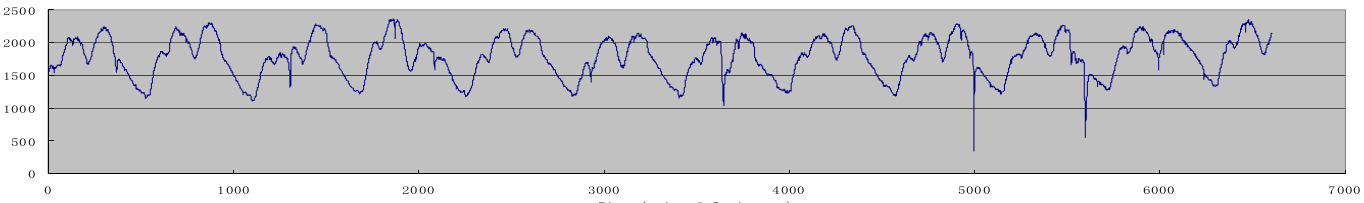
\includegraphics[width=1\textwidth]{img/connection_peer_hour.png}
  \label{fig:conection_peer_hour}
\end{figure}

Os serviços escritos atualmente, a qual podem suportar suportar milhares de jogadores, estão trabalhando como microserviços\cite{stephenclarkewillson2017}\cite{albion_online_unite}. Estes microserviços são pequenos softwares que realizam uma determinada ação de forma exemplar, uma evolução do conceito de utilidades Unix "\textit{doing one thing well}". Esses serviços pertencem a uma coleção de serviços denominada macroserviço, a qual corresponde ao serviço completo de backend da aplicação.

Os microserviços para estado de jogo são separados conforme a posição virtual do personagem do jogador. Dessa forma, regiões mais visitadas por jogadores terão maior tráfego de rede e consumo de recursos comparados a regiões pouco exploradas. Esta é uma perca grande de recurso atualmente existente nessa arquitetura \cite{cloud_fog}.
